\documentclass[compress]{beamer}
\usepackage[utf8]{inputenc}
\usepackage[T1]{fontenc}
\usepackage{lmodern}
\usepackage[french]{babel}
\usepackage{amsfonts}
\usepackage{amsmath}
\usepackage{amsthm}

\useinnertheme{default}
\useoutertheme{miniframes}
\usecolortheme{beaver}
\setbeamercovered{transparent}
\setbeamertemplate{section in toc}[sections numbered]

\newcommand{\cont}{\mathcal{C}^0}
\newcommand{\cun}{\mathcal{C}^1}
\newcommand{\cinf}{\mathcal{C}^\infty}
\newcommand{\R}{\mathbb{R}}
\newcommand{\N}{\mathbb{N}}

\newtheorem{thm}{Théorème}
\newtheorem{lemm}{Lemme}
\theoremstyle{definition}
\newtheorem{defn}{Définition}

\author{Farid Arthaud}
\title{Théorie des Catastrophes}
\date{\today}

\begin{document}
\section*{Introduction}

\frame{\titlepage}

\frame{\tableofcontents}

\begin{frame}{Contexte historique}
    \begin{itemize}
        \item Hassler \textsc{Whitney}: classification pour les dimensions inférieures à deux (1955)
        \item René \textsc{Thom}: \textit{Stabilité structurelle et morphogenèse} (1972)
        \item Cristopher \textsc{Zeeman}: Recherche intensive aux cotés de \textsc{Thom}
        \item Popularisation (années 70) et applications diverses (biologie, sociologie, ...)
        \item Controverse, remise en question de la pertinence des applications
    \end{itemize}
    \begin{quote}<2>
        ``Les choses qui changent soudainement, par à-coups, ont longtemps résisté à toute analyse mathématique.
        Une méthode dérivée de la topologie décrit ces phénomènes comme des exemples de sept `catastrophes élémentaires'.'' - C. \textsc{Zeeman}
    \end{quote}
\end{frame}

\begin{frame}{Exemple: le baigneur}
    \begin{columns}[T]
        \begin{column}{5cm}
            \begin{itemize}[<+->]
                \item Contrôle absolu sur la précision
                \item `Virage' soudain et incontournable lors du réglage du paramètre
            \end{itemize}

            \pause[3]
            \alert{Explication}: Disparition d'un équilibre d'un système physique caché dont la température est une projection

            \pause[4]
            \alert{Objectif}: Saisir la classification des catastrophes établie par \textsc{Thom} en faibles dimensions, et ses applications
        \end{column}
        \begin{column}{5cm}
            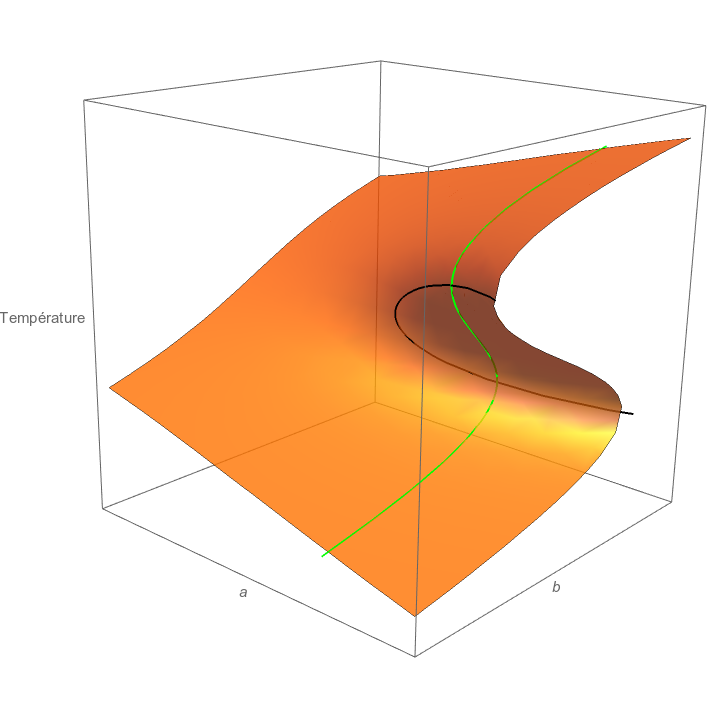
\includegraphics[width=\linewidth,height=0.8\textheight,keepaspectratio]{images/cusp_temp.png}
        \end{column}
    \end{columns}
\end{frame}

\section{Premiers exemples}

\subsection{La machine de \textsc{Zeeman}}
\begin{frame}{Expérience}
    \includegraphics<1>[width=\linewidth,height=\textheight,keepaspectratio]{images/montage_loq.jpg}
    \includegraphics<2>[width=\linewidth,height=\textheight,keepaspectratio]{images/eq_haut_loq.jpg}
    \includegraphics<3>[width=\linewidth,height=\textheight,keepaspectratio]{images/eq_bas_loq.jpg}
\end{frame}

\begin{frame}{Analyse théorique}
    \begin{onlyenv}<1>
        On change de coordonnées, $x=\theta+c$, un calcul donne:

        $$E_p(x)  = \frac{1}{4}x^4+\frac{a}{2}x^2+bx$$


        \alert{Points critiques} ou positions d'équilibre:

        $$x^3+ax+b=0$$
    \end{onlyenv}

    \includegraphics<2>[width=\linewidth,height=0.8\textheight,keepaspectratio]{images/cusp_zeeman.png}
    \includegraphics<3>[width=\linewidth,height=0.8\textheight,keepaspectratio]{images/cusp_side.png}
\end{frame}

\subsection{Surface en trois dimensions}
\begin{frame}{Points-pli et points-fronce}
    On s'intéresse à $f:\R^3\to\R, \cinf$ et à la surface $V=ker(f)\subseteq \R^3$

    \begin{columns}[T]
        \begin{column}{5cm}
            \alert{Point-pli}

            $a$ est point-pli s'il existe des coordonnées dans lesquelles

            $$\pm f = z^2 - y$$

            \uncover<3>{
                \alert{Point-fronce}

                $a$ est point-fronce s'il existe des coordonnées dans lesquelles

                $$\pm f = z^3 - xz - y$$}
        \end{column}
        \begin{column}{5cm}
            \includegraphics<1>[width=5cm,keepaspectratio]{images/fold_front.png}
            \includegraphics<2>[width=5cm,keepaspectratio]{images/fold_side.png}
            \includegraphics<3>[width=5cm,keepaspectratio]{images/cusp_front.png}
        \end{column}
    \end{columns}
\end{frame}

\begin{frame}{Contour d'une surface}
    On projette sur $\R^2$, le contour apparent est l'ensemble des points de la surface où $\frac{\partial f}{\partial z}=0$

    \begin{thm}
        Si $f$ est générique, alors:
        \begin{enumerate}[<+->]
            \item $ker(f)$ est une sous-variété de dimension deux (\alert{surface})
            \item Son contour apparent $ker(f)\cap ker(\frac{\partial f}{\partial z})$ est une sous-variété de dimension un (\alert{courbe})
            \item Tous les points sont des points-plis ou points-fronces, les points-fronces sont isolés
        \end{enumerate}
    \end{thm}

    \pause[4]
    \begin{proof}
        Appliquer le théorème de transversalité à $j^1f: \R^3 \to J^2(\R^3,\R) \simeq \R^{13}$
    \end{proof}
\end{frame}

\section{Catastrophes}

\subsection{Variétés et points critiques}
\begin{frame}{Points critiques}
    Soit $f: E \to F, \cinf$
    \begin{defn}
        Un point critique pour $f$ est un point $a$ où $df_a$ n'est \alert{pas surjective}.

	    Un point critique $a$ est dit \textbf{non dégénéré} si $\forall x, d^2f_a(x)$ est un \alert{isomorphisme}, ou de manière équivalente si le déterminant Hessien de $f$ est non nul.
    \end{defn}

    \pause
    En \textbf{dimension 1}: $a$ point critique $\iff f'(a) = 0$

    $a$ point critique dégénéré $\iff f'(a) =f''(a) = 0$
\end{frame}

\begin{frame}{Sous-variétés}
    \begin{defn}
        Une \textbf{sous-variété} $V$ de $\R^n$ est un ensemble qui est localement descriptible par un \alert{système non dégénéré d'équations locales}, soit $m$ équations indépendantes.
        \begin{enumerate}[<+->]
            \item pour un voisinage $U$ de $a$, $U\cap\ker(\Phi_1,...,\Phi_m)=U\cap V$
            \item $d\Phi_1,...,d\Phi_m$ forment un système libre de formes linéaires.
        \end{enumerate}
        \pause[3]
        $m$ s'appelle la \textbf{codimension} de la sous-variété, que l'on suppose être la même en tout point de $V$ par la suite (on peut supposer la variété connexe par exemple).
    \end{defn}

    \pause[4]
    \begin{thm}
        Une variété de dimension $p$ admet en tout point un \alert{espace tangent} de dimension $p$.

        C'est en fait l'intersection transverse des $d\phi_1,...,d\phi_m$.
    \end{thm}
\end{frame}

\subsection{Transversalité et généricité}
\begin{frame}{Intersections transverses}
    \begin{defn}
        Deux sous-espaces $F$ et $G$ sont dits d'\textbf{intersection transverse} si $F+G=E$.
    \end{defn}

    \pause
    Caractérisations:
    \begin{enumerate}
        \item<2-> Intersection minimale
        \item<2-> Tous sous-espaces affines parallèles s'intersectent
        \item<3-> $dim(F\cap G)=dim(F)+dim(G)-dim(E)$
        \item<3-> $codim(F\cap G)=codim(F)+codim(G)$
    \end{enumerate}

    \pause[4]
    Pour des variétés et des fonctions, transversalité si les espaces tangents transverses en tout point de l'intersection
\end{frame}

\begin{frame}{Théorèmes de transversalité}
    \begin{thm}
        Une intersection transverse de sous-variétés est une sous-variété.
    \end{thm}
    \pause
    Soit $g:V\to W, \cinf$
    \begin{thm}
        Si $a\in g^{-1}(W)$ et $g$ transverse à $W$ en $a$, alors $g^{-1}(W)$ est sous-variété en $a$ de dimension $dim_a(V)-codim_{g(a)}(W)$.
    \end{thm}

    \pause
    Choix ``au hasard'': par densité.
    Notion de \alert{généricité}.

    \pause
    \begin{thm}{(de transversalité faible)}
        Si $X$ est une sous-variété de $W$, une application $V\to W$ choisie ``au hasard'' (par généricité) sera transverse à $W$.
    \end{thm}
\end{frame}

\subsection{Germes et jets}
\begin{frame}{Espace des germes}
    \begin{defn}
        Un \textbf{$k$-jet} de $f$ en $x$ correspond aux premiers termes du développement de Taylor d'une fonction.

        $$(j^k_x f)(h) = f(x) + df_x(h)+...+\frac{df^k_x(h)(h)...(h)}{k!}$$

        L'\textbf{espace des germes} correspond aux couples $(a, j_af)$
    \end{defn}

    \pause
    Permet d'exprimer des \textit{équations différentielles} comme des variétés:

    $$f'(x)=f(x) \iff (x,j^1_xf) \in \{(a,b,c) \mid b=c \} \subseteq J^1(\R,\R) \simeq \R^3$$
\end{frame}

\section{Théorème de classification}

\subsection{Théorème de transversalité de \textsc{Thom}}
\begin{frame}{Le théorème de transversalité de \textsc{Thom}}
    \begin{thm}{(de transversalité de \textsc{Thom})}
        Pour une sous-variété $W$ d'un espace des germes $J^r(E,F)$ donnée, une fonction $f$ choisie ``au hasard'' (par densité) aura $j^rf$ transverse à $W$.
    \end{thm}

    \pause
    \textbf{Exemple}: $\{(a,b,c) \mid b=c \}$ est une sous-variété de dimension $2$ de $J^1(\R,\R)$ décrivant $f'=f$

    \pause
    Espace tangent en $(a,b,b)$: $\left((1,0,0), (0,1,1)\right)$

    Espace tangent de $j^1f$ en $j^1_xf$: $(1,f'(x),f''(x))\notin\left((1,0,0), (0,1,1)\right)$

    \pause
    Une fonction $f$ choisie ``au hasard'' en chaque point soit: ne vérifie pas $f'(x)=f(x)$, soit la vérifie en un point isolé
\end{frame}

\subsection{Le pli et la fronce}
\begin{frame}{Théorème de \textsc{Whitney}}
    On s'intéresse cette fois-ci aux fonctions $f: \R^2 \to \R^2$ (son graphe est une hypersurface de $\R^4$)

    \pause
    \alert{Point-pli}: il existe des coordonnées $(x',y')$ en $f(a)$ dans lesquelles $x' = x, y' = y^2$

    \pause
    \alert{Point-fronce}: il existe des coordonnées $(x',y')$ en $f(a)$ dans lesquelles $x' = x, y' = y^3 - xy$

    \pause
    \begin{thm}{(de \textsc{Whitney})}
        Si $f$ est choisie ``au hasard'', alors:
        \begin{enumerate}[<+->]
            \item Les points critiques de $f$ forment une sous-variété de dimension une (\alert{courbe})
            \item Les points critiques sont des plis et des fronces
            \item Les fronces sont isolées
        \end{enumerate}
    \end{thm}
\end{frame}

\subsection{Les autres catastrophes}
\begin{frame}{Le théorème de classification}
    Si $f:\R^n\to\R$, il existe des coordonnées au voisinage d'un point critique telles que:

    $$\begin{cases}f  - f(a) = \pm x_1^{r+1} + \sum \pm x_i^2 & \text{pour } 1\leq r\leq 5 \\
    f - f(a) =  x_1^2x_2 \pm x_2^{r-1} + \sum \pm x_i^2 & \text{pour } r=4,5 \end{cases}$$

    \pause
    \begin{description}[Ombilic hyperbolique]
        \item[Pli] $x^3$
        \item[Fronce] $\pm x^4$
        \item[Queue d'aronde] $x^5$
        \item[Papillon] $x^6$
        \item[Ombilic hyperbolique] $x^2y+y^3$
        \item[Ombilic elliptique] $x^2y-y^3$
        \item[Ombilic parabolique] $x^2y \pm y^4$
    \end{description}
\end{frame}

\end{document}

\subsection{Réecriture au voisinage d'un point critique}
\begin{frame}{Lemmes d'\textsc{Hadamard}, de \textsc{Morse}, inversion locale}
    \begin{thm}{(inversion locale)}
        Si $a$ n'est pas un point critique, il existe des coordonnées locales telles que $f(x)=f(a)+x$.
    \end{thm}
    \begin{lemm}{(de \textsc{Hadamard})}
        Il existe un voisinage de $0$ sur lequel $f$ peut s'écrire: $f(x)=x_1g_1(x)+...+x_ng_n(x)$ avec $g_i(0) = \frac{\partial f}{\partial x_i}(0)$.

        Si $df_0=0$, on peut réitérer cela et écrire (toujours sur un voisinage de $0$):

        $$f(x)=\sum_{1\leq i,j \leq n} x_ix_jh_{ij}(x)$$
    \end{lemm}
    \begin{lemm}{(de \textsc{Morse})}
        Si $f$ admet un point critique non dégénéré en $u$, alors il existe un voisinage de $u$ et des coordonnées centrées en $u$ $y=(y_1,...,y_n)$ tels que:

        $$f=f(u)+y_1^2+...+y_l^2-y_{l+1}^2-...-y_n^2$$

        $l$ ne dépend pas des coordonnées choisies.
    \end{lemm}
\end{frame}

\includegraphics[width=5cm,keepaspectratio]{images/others.jpg}
